% Created by tikzDevice version 0.12 on 2019-05-23 20:16:36
% !TEX encoding = UTF-8 Unicode
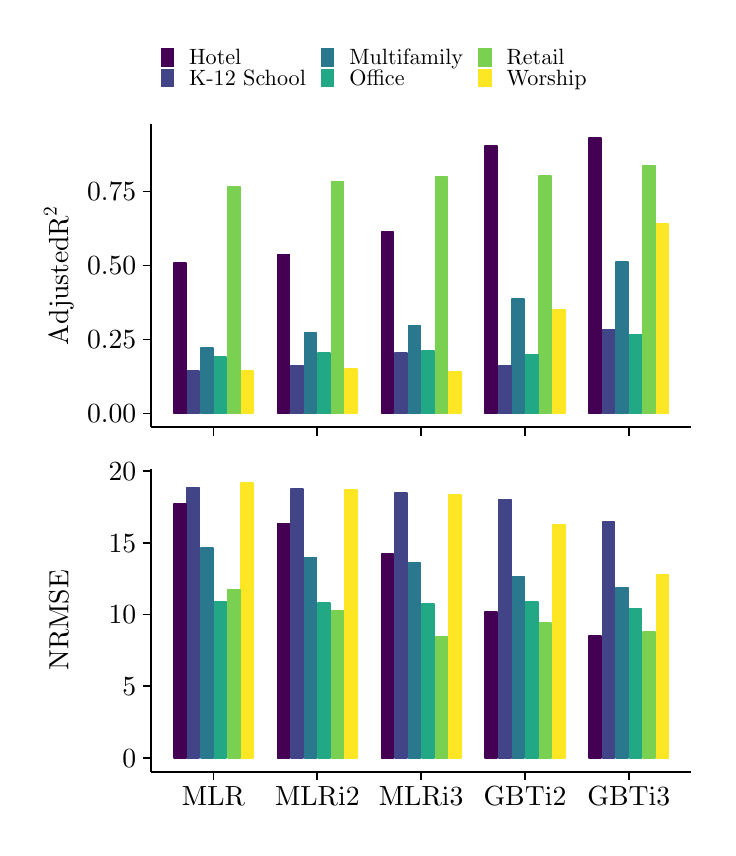
\begin{tikzpicture}[x=1pt,y=1pt]
\definecolor{fillColor}{RGB}{255,255,255}
\path[use as bounding box,fill=fillColor,fill opacity=0.00] (0,0) rectangle (245.72,289.08);
\begin{scope}
\path[clip] (  0.00,135.70) rectangle (245.72,289.08);
\definecolor{drawColor}{RGB}{255,255,255}
\definecolor{fillColor}{RGB}{255,255,255}

\path[draw=drawColor,line width= 0.6pt,line join=round,line cap=round,fill=fillColor] (  0.00,135.70) rectangle (245.72,289.08);
\end{scope}
\begin{scope}
\path[clip] (  0.00,  0.00) rectangle (245.72,135.70);
\definecolor{drawColor}{RGB}{255,255,255}
\definecolor{fillColor}{RGB}{255,255,255}

\path[draw=drawColor,line width= 0.6pt,line join=round,line cap=round,fill=fillColor] (  0.00,  0.00) rectangle (245.72,135.70);
\end{scope}
\begin{scope}
\path[clip] ( 44.64,144.70) rectangle (239.72,254.17);
\definecolor{fillColor}{RGB}{255,255,255}

\path[fill=fillColor] ( 44.64,144.70) rectangle (239.72,254.17);
\definecolor{drawColor}{RGB}{253,231,37}
\definecolor{fillColor}{RGB}{253,231,37}

\path[draw=drawColor,line width= 0.6pt,line join=round,fill=fillColor] ( 77.15,149.68) rectangle ( 81.53,165.19);
\definecolor{drawColor}{RGB}{122,209,81}
\definecolor{fillColor}{RGB}{122,209,81}

\path[draw=drawColor,line width= 0.6pt,line join=round,fill=fillColor] ( 72.28,149.68) rectangle ( 76.65,231.65);
\definecolor{drawColor}{RGB}{34,168,132}
\definecolor{fillColor}{RGB}{34,168,132}

\path[draw=drawColor,line width= 0.6pt,line join=round,fill=fillColor] ( 67.40,149.68) rectangle ( 71.78,170.12);
\definecolor{drawColor}{RGB}{42,120,142}
\definecolor{fillColor}{RGB}{42,120,142}

\path[draw=drawColor,line width= 0.6pt,line join=round,fill=fillColor] ( 62.52,149.68) rectangle ( 66.90,173.22);
\definecolor{drawColor}{RGB}{65,68,135}
\definecolor{fillColor}{RGB}{65,68,135}

\path[draw=drawColor,line width= 0.6pt,line join=round,fill=fillColor] ( 57.65,149.68) rectangle ( 62.02,165.09);
\definecolor{drawColor}{RGB}{68,1,84}
\definecolor{fillColor}{RGB}{68,1,84}

\path[draw=drawColor,line width= 0.6pt,line join=round,fill=fillColor] ( 52.77,149.68) rectangle ( 57.15,203.93);
\definecolor{drawColor}{RGB}{253,231,37}
\definecolor{fillColor}{RGB}{253,231,37}

\path[draw=drawColor,line width= 0.6pt,line join=round,fill=fillColor] (114.67,149.68) rectangle (119.05,165.84);
\definecolor{drawColor}{RGB}{122,209,81}
\definecolor{fillColor}{RGB}{122,209,81}

\path[draw=drawColor,line width= 0.6pt,line join=round,fill=fillColor] (109.79,149.68) rectangle (114.17,233.47);
\definecolor{drawColor}{RGB}{34,168,132}
\definecolor{fillColor}{RGB}{34,168,132}

\path[draw=drawColor,line width= 0.6pt,line join=round,fill=fillColor] (104.91,149.68) rectangle (109.29,171.51);
\definecolor{drawColor}{RGB}{42,120,142}
\definecolor{fillColor}{RGB}{42,120,142}

\path[draw=drawColor,line width= 0.6pt,line join=round,fill=fillColor] (100.04,149.68) rectangle (104.41,178.78);
\definecolor{drawColor}{RGB}{65,68,135}
\definecolor{fillColor}{RGB}{65,68,135}

\path[draw=drawColor,line width= 0.6pt,line join=round,fill=fillColor] ( 95.16,149.68) rectangle ( 99.54,167.01);
\definecolor{drawColor}{RGB}{68,1,84}
\definecolor{fillColor}{RGB}{68,1,84}

\path[draw=drawColor,line width= 0.6pt,line join=round,fill=fillColor] ( 90.28,149.68) rectangle ( 94.66,207.14);
\definecolor{drawColor}{RGB}{253,231,37}
\definecolor{fillColor}{RGB}{253,231,37}

\path[draw=drawColor,line width= 0.6pt,line join=round,fill=fillColor] (152.18,149.68) rectangle (156.56,164.87);
\definecolor{drawColor}{RGB}{122,209,81}
\definecolor{fillColor}{RGB}{122,209,81}

\path[draw=drawColor,line width= 0.6pt,line join=round,fill=fillColor] (147.31,149.68) rectangle (151.68,235.18);
\definecolor{drawColor}{RGB}{34,168,132}
\definecolor{fillColor}{RGB}{34,168,132}

\path[draw=drawColor,line width= 0.6pt,line join=round,fill=fillColor] (142.43,149.68) rectangle (146.81,172.36);
\definecolor{drawColor}{RGB}{42,120,142}
\definecolor{fillColor}{RGB}{42,120,142}

\path[draw=drawColor,line width= 0.6pt,line join=round,fill=fillColor] (137.55,149.68) rectangle (141.93,181.46);
\definecolor{drawColor}{RGB}{65,68,135}
\definecolor{fillColor}{RGB}{65,68,135}

\path[draw=drawColor,line width= 0.6pt,line join=round,fill=fillColor] (132.68,149.68) rectangle (137.05,171.61);
\definecolor{drawColor}{RGB}{68,1,84}
\definecolor{fillColor}{RGB}{68,1,84}

\path[draw=drawColor,line width= 0.6pt,line join=round,fill=fillColor] (127.80,149.68) rectangle (132.18,215.27);
\definecolor{drawColor}{RGB}{253,231,37}
\definecolor{fillColor}{RGB}{253,231,37}

\path[draw=drawColor,line width= 0.6pt,line join=round,fill=fillColor] (189.70,149.68) rectangle (194.08,187.24);
\definecolor{drawColor}{RGB}{122,209,81}
\definecolor{fillColor}{RGB}{122,209,81}

\path[draw=drawColor,line width= 0.6pt,line join=round,fill=fillColor] (184.82,149.68) rectangle (189.20,235.39);
\definecolor{drawColor}{RGB}{34,168,132}
\definecolor{fillColor}{RGB}{34,168,132}

\path[draw=drawColor,line width= 0.6pt,line join=round,fill=fillColor] (179.94,149.68) rectangle (184.32,170.97);
\definecolor{drawColor}{RGB}{42,120,142}
\definecolor{fillColor}{RGB}{42,120,142}

\path[draw=drawColor,line width= 0.6pt,line join=round,fill=fillColor] (175.07,149.68) rectangle (179.44,191.09);
\definecolor{drawColor}{RGB}{65,68,135}
\definecolor{fillColor}{RGB}{65,68,135}

\path[draw=drawColor,line width= 0.6pt,line join=round,fill=fillColor] (170.19,149.68) rectangle (174.57,166.91);
\definecolor{drawColor}{RGB}{68,1,84}
\definecolor{fillColor}{RGB}{68,1,84}

\path[draw=drawColor,line width= 0.6pt,line join=round,fill=fillColor] (165.31,149.68) rectangle (169.69,246.31);
\definecolor{drawColor}{RGB}{253,231,37}
\definecolor{fillColor}{RGB}{253,231,37}

\path[draw=drawColor,line width= 0.6pt,line join=round,fill=fillColor] (227.21,149.68) rectangle (231.59,218.06);
\definecolor{drawColor}{RGB}{122,209,81}
\definecolor{fillColor}{RGB}{122,209,81}

\path[draw=drawColor,line width= 0.6pt,line join=round,fill=fillColor] (222.34,149.68) rectangle (226.71,239.24);
\definecolor{drawColor}{RGB}{34,168,132}
\definecolor{fillColor}{RGB}{34,168,132}

\path[draw=drawColor,line width= 0.6pt,line join=round,fill=fillColor] (217.46,149.68) rectangle (221.84,178.25);
\definecolor{drawColor}{RGB}{42,120,142}
\definecolor{fillColor}{RGB}{42,120,142}

\path[draw=drawColor,line width= 0.6pt,line join=round,fill=fillColor] (212.58,149.68) rectangle (216.96,204.36);
\definecolor{drawColor}{RGB}{65,68,135}
\definecolor{fillColor}{RGB}{65,68,135}

\path[draw=drawColor,line width= 0.6pt,line join=round,fill=fillColor] (207.71,149.68) rectangle (212.08,180.07);
\definecolor{drawColor}{RGB}{68,1,84}
\definecolor{fillColor}{RGB}{68,1,84}

\path[draw=drawColor,line width= 0.6pt,line join=round,fill=fillColor] (202.83,149.68) rectangle (207.21,249.20);
\end{scope}
\begin{scope}
\path[clip] ( 44.64, 20.23) rectangle (239.72,129.70);
\definecolor{fillColor}{RGB}{255,255,255}

\path[fill=fillColor] ( 44.64, 20.23) rectangle (239.72,129.70);
\definecolor{drawColor}{RGB}{253,231,37}
\definecolor{fillColor}{RGB}{253,231,37}

\path[draw=drawColor,line width= 0.6pt,line join=round,fill=fillColor] ( 77.15, 25.21) rectangle ( 81.53,124.73);
\definecolor{drawColor}{RGB}{122,209,81}
\definecolor{fillColor}{RGB}{122,209,81}

\path[draw=drawColor,line width= 0.6pt,line join=round,fill=fillColor] ( 72.28, 25.21) rectangle ( 76.65, 86.03);
\definecolor{drawColor}{RGB}{34,168,132}
\definecolor{fillColor}{RGB}{34,168,132}

\path[draw=drawColor,line width= 0.6pt,line join=round,fill=fillColor] ( 67.40, 25.21) rectangle ( 71.78, 81.71);
\definecolor{drawColor}{RGB}{42,120,142}
\definecolor{fillColor}{RGB}{42,120,142}

\path[draw=drawColor,line width= 0.6pt,line join=round,fill=fillColor] ( 62.52, 25.21) rectangle ( 66.90,101.17);
\definecolor{drawColor}{RGB}{65,68,135}
\definecolor{fillColor}{RGB}{65,68,135}

\path[draw=drawColor,line width= 0.6pt,line join=round,fill=fillColor] ( 57.65, 25.21) rectangle ( 62.02,122.93);
\definecolor{drawColor}{RGB}{68,1,84}
\definecolor{fillColor}{RGB}{68,1,84}

\path[draw=drawColor,line width= 0.6pt,line join=round,fill=fillColor] ( 52.77, 25.21) rectangle ( 57.15,117.02);
\definecolor{drawColor}{RGB}{253,231,37}
\definecolor{fillColor}{RGB}{253,231,37}

\path[draw=drawColor,line width= 0.6pt,line join=round,fill=fillColor] (114.67, 25.21) rectangle (119.05,122.11);
\definecolor{drawColor}{RGB}{122,209,81}
\definecolor{fillColor}{RGB}{122,209,81}

\path[draw=drawColor,line width= 0.6pt,line join=round,fill=fillColor] (109.79, 25.21) rectangle (114.17, 78.36);
\definecolor{drawColor}{RGB}{34,168,132}
\definecolor{fillColor}{RGB}{34,168,132}

\path[draw=drawColor,line width= 0.6pt,line join=round,fill=fillColor] (104.91, 25.21) rectangle (109.29, 81.21);
\definecolor{drawColor}{RGB}{42,120,142}
\definecolor{fillColor}{RGB}{42,120,142}

\path[draw=drawColor,line width= 0.6pt,line join=round,fill=fillColor] (100.04, 25.21) rectangle (104.41, 97.66);
\definecolor{drawColor}{RGB}{65,68,135}
\definecolor{fillColor}{RGB}{65,68,135}

\path[draw=drawColor,line width= 0.6pt,line join=round,fill=fillColor] ( 95.16, 25.21) rectangle ( 99.54,122.47);
\definecolor{drawColor}{RGB}{68,1,84}
\definecolor{fillColor}{RGB}{68,1,84}

\path[draw=drawColor,line width= 0.6pt,line join=round,fill=fillColor] ( 90.28, 25.21) rectangle ( 94.66,109.90);
\definecolor{drawColor}{RGB}{253,231,37}
\definecolor{fillColor}{RGB}{253,231,37}

\path[draw=drawColor,line width= 0.6pt,line join=round,fill=fillColor] (152.18, 25.21) rectangle (156.56,120.37);
\definecolor{drawColor}{RGB}{122,209,81}
\definecolor{fillColor}{RGB}{122,209,81}

\path[draw=drawColor,line width= 0.6pt,line join=round,fill=fillColor] (147.31, 25.21) rectangle (151.68, 68.82);
\definecolor{drawColor}{RGB}{34,168,132}
\definecolor{fillColor}{RGB}{34,168,132}

\path[draw=drawColor,line width= 0.6pt,line join=round,fill=fillColor] (142.43, 25.21) rectangle (146.81, 80.76);
\definecolor{drawColor}{RGB}{42,120,142}
\definecolor{fillColor}{RGB}{42,120,142}

\path[draw=drawColor,line width= 0.6pt,line join=round,fill=fillColor] (137.55, 25.21) rectangle (141.93, 95.62);
\definecolor{drawColor}{RGB}{65,68,135}
\definecolor{fillColor}{RGB}{65,68,135}

\path[draw=drawColor,line width= 0.6pt,line join=round,fill=fillColor] (132.68, 25.21) rectangle (137.05,120.99);
\definecolor{drawColor}{RGB}{68,1,84}
\definecolor{fillColor}{RGB}{68,1,84}

\path[draw=drawColor,line width= 0.6pt,line join=round,fill=fillColor] (127.80, 25.21) rectangle (132.18, 98.82);
\definecolor{drawColor}{RGB}{253,231,37}
\definecolor{fillColor}{RGB}{253,231,37}

\path[draw=drawColor,line width= 0.6pt,line join=round,fill=fillColor] (189.70, 25.21) rectangle (194.08,109.50);
\definecolor{drawColor}{RGB}{122,209,81}
\definecolor{fillColor}{RGB}{122,209,81}

\path[draw=drawColor,line width= 0.6pt,line join=round,fill=fillColor] (184.82, 25.21) rectangle (189.20, 74.05);
\definecolor{drawColor}{RGB}{34,168,132}
\definecolor{fillColor}{RGB}{34,168,132}

\path[draw=drawColor,line width= 0.6pt,line join=round,fill=fillColor] (179.94, 25.21) rectangle (184.32, 81.44);
\definecolor{drawColor}{RGB}{42,120,142}
\definecolor{fillColor}{RGB}{42,120,142}

\path[draw=drawColor,line width= 0.6pt,line join=round,fill=fillColor] (175.07, 25.21) rectangle (179.44, 90.82);
\definecolor{drawColor}{RGB}{65,68,135}
\definecolor{fillColor}{RGB}{65,68,135}

\path[draw=drawColor,line width= 0.6pt,line join=round,fill=fillColor] (170.19, 25.21) rectangle (174.57,118.54);
\definecolor{drawColor}{RGB}{68,1,84}
\definecolor{fillColor}{RGB}{68,1,84}

\path[draw=drawColor,line width= 0.6pt,line join=round,fill=fillColor] (165.31, 25.21) rectangle (169.69, 77.96);
\definecolor{drawColor}{RGB}{253,231,37}
\definecolor{fillColor}{RGB}{253,231,37}

\path[draw=drawColor,line width= 0.6pt,line join=round,fill=fillColor] (227.21, 25.21) rectangle (231.59, 91.22);
\definecolor{drawColor}{RGB}{122,209,81}
\definecolor{fillColor}{RGB}{122,209,81}

\path[draw=drawColor,line width= 0.6pt,line join=round,fill=fillColor] (222.34, 25.21) rectangle (226.71, 70.82);
\definecolor{drawColor}{RGB}{34,168,132}
\definecolor{fillColor}{RGB}{34,168,132}

\path[draw=drawColor,line width= 0.6pt,line join=round,fill=fillColor] (217.46, 25.21) rectangle (221.84, 79.08);
\definecolor{drawColor}{RGB}{42,120,142}
\definecolor{fillColor}{RGB}{42,120,142}

\path[draw=drawColor,line width= 0.6pt,line join=round,fill=fillColor] (212.58, 25.21) rectangle (216.96, 86.74);
\definecolor{drawColor}{RGB}{65,68,135}
\definecolor{fillColor}{RGB}{65,68,135}

\path[draw=drawColor,line width= 0.6pt,line join=round,fill=fillColor] (207.71, 25.21) rectangle (212.08,110.53);
\definecolor{drawColor}{RGB}{68,1,84}
\definecolor{fillColor}{RGB}{68,1,84}

\path[draw=drawColor,line width= 0.6pt,line join=round,fill=fillColor] (202.83, 25.21) rectangle (207.21, 69.36);
\end{scope}
\begin{scope}
\path[clip] (  0.00,  0.00) rectangle (245.72,289.08);
\definecolor{drawColor}{RGB}{0,0,0}

\path[draw=drawColor,line width= 0.6pt,line join=round] ( 44.64,144.70) --
	( 44.64,254.17);
\end{scope}
\begin{scope}
\path[clip] (  0.00,  0.00) rectangle (245.72,289.08);
\definecolor{drawColor}{RGB}{0,0,0}

\node[text=drawColor,anchor=base east,inner sep=0pt, outer sep=0pt, scale=  1.00] at ( 39.24,146.23) {0.00};

\node[text=drawColor,anchor=base east,inner sep=0pt, outer sep=0pt, scale=  1.00] at ( 39.24,172.99) {0.25};

\node[text=drawColor,anchor=base east,inner sep=0pt, outer sep=0pt, scale=  1.00] at ( 39.24,199.74) {0.50};

\node[text=drawColor,anchor=base east,inner sep=0pt, outer sep=0pt, scale=  1.00] at ( 39.24,226.49) {0.75};
\end{scope}
\begin{scope}
\path[clip] (  0.00,  0.00) rectangle (245.72,289.08);
\definecolor{drawColor}{RGB}{0,0,0}

\path[draw=drawColor,line width= 0.6pt,line join=round] ( 41.64,149.68) --
	( 44.64,149.68);

\path[draw=drawColor,line width= 0.6pt,line join=round] ( 41.64,176.43) --
	( 44.64,176.43);

\path[draw=drawColor,line width= 0.6pt,line join=round] ( 41.64,203.18) --
	( 44.64,203.18);

\path[draw=drawColor,line width= 0.6pt,line join=round] ( 41.64,229.93) --
	( 44.64,229.93);
\end{scope}
\begin{scope}
\path[clip] (  0.00,  0.00) rectangle (245.72,289.08);
\definecolor{drawColor}{RGB}{0,0,0}

\path[draw=drawColor,line width= 0.6pt,line join=round] ( 44.64, 20.23) --
	( 44.64,129.70);
\end{scope}
\begin{scope}
\path[clip] (  0.00,  0.00) rectangle (245.72,289.08);
\definecolor{drawColor}{RGB}{0,0,0}

\node[text=drawColor,anchor=base east,inner sep=0pt, outer sep=0pt, scale=  1.00] at ( 39.24, 21.76) {0};

\node[text=drawColor,anchor=base east,inner sep=0pt, outer sep=0pt, scale=  1.00] at ( 39.24, 47.68) {5};

\node[text=drawColor,anchor=base east,inner sep=0pt, outer sep=0pt, scale=  1.00] at ( 39.24, 73.60) {10};

\node[text=drawColor,anchor=base east,inner sep=0pt, outer sep=0pt, scale=  1.00] at ( 39.24, 99.52) {15};

\node[text=drawColor,anchor=base east,inner sep=0pt, outer sep=0pt, scale=  1.00] at ( 39.24,125.44) {20};
\end{scope}
\begin{scope}
\path[clip] (  0.00,  0.00) rectangle (245.72,289.08);
\definecolor{drawColor}{RGB}{0,0,0}

\path[draw=drawColor,line width= 0.6pt,line join=round] ( 41.64, 25.21) --
	( 44.64, 25.21);

\path[draw=drawColor,line width= 0.6pt,line join=round] ( 41.64, 51.13) --
	( 44.64, 51.13);

\path[draw=drawColor,line width= 0.6pt,line join=round] ( 41.64, 77.05) --
	( 44.64, 77.05);

\path[draw=drawColor,line width= 0.6pt,line join=round] ( 41.64,102.96) --
	( 44.64,102.96);

\path[draw=drawColor,line width= 0.6pt,line join=round] ( 41.64,128.88) --
	( 44.64,128.88);
\end{scope}
\begin{scope}
\path[clip] (  0.00,  0.00) rectangle (245.72,289.08);
\definecolor{drawColor}{RGB}{0,0,0}

\path[draw=drawColor,line width= 0.6pt,line join=round] ( 44.64,144.70) --
	(239.72,144.70);
\end{scope}
\begin{scope}
\path[clip] (  0.00,  0.00) rectangle (245.72,289.08);
\definecolor{drawColor}{RGB}{0,0,0}

\path[draw=drawColor,line width= 0.6pt,line join=round] ( 67.15,141.70) --
	( 67.15,144.70);

\path[draw=drawColor,line width= 0.6pt,line join=round] (104.66,141.70) --
	(104.66,144.70);

\path[draw=drawColor,line width= 0.6pt,line join=round] (142.18,141.70) --
	(142.18,144.70);

\path[draw=drawColor,line width= 0.6pt,line join=round] (179.69,141.70) --
	(179.69,144.70);

\path[draw=drawColor,line width= 0.6pt,line join=round] (217.21,141.70) --
	(217.21,144.70);
\end{scope}
\begin{scope}
\path[clip] (  0.00,  0.00) rectangle (245.72,289.08);
\definecolor{drawColor}{RGB}{0,0,0}

\path[draw=drawColor,line width= 0.6pt,line join=round] ( 44.64, 20.23) --
	(239.72, 20.23);
\end{scope}
\begin{scope}
\path[clip] (  0.00,  0.00) rectangle (245.72,289.08);
\definecolor{drawColor}{RGB}{0,0,0}

\path[draw=drawColor,line width= 0.6pt,line join=round] ( 67.15, 17.23) --
	( 67.15, 20.23);

\path[draw=drawColor,line width= 0.6pt,line join=round] (104.66, 17.23) --
	(104.66, 20.23);

\path[draw=drawColor,line width= 0.6pt,line join=round] (142.18, 17.23) --
	(142.18, 20.23);

\path[draw=drawColor,line width= 0.6pt,line join=round] (179.69, 17.23) --
	(179.69, 20.23);

\path[draw=drawColor,line width= 0.6pt,line join=round] (217.21, 17.23) --
	(217.21, 20.23);
\end{scope}
\begin{scope}
\path[clip] (  0.00,  0.00) rectangle (245.72,289.08);
\definecolor{drawColor}{RGB}{0,0,0}

\node[text=drawColor,anchor=base,inner sep=0pt, outer sep=0pt, scale=  1.00] at ( 67.15,  7.94) {MLR};

\node[text=drawColor,anchor=base,inner sep=0pt, outer sep=0pt, scale=  1.00] at (104.66,  7.94) {MLRi2};

\node[text=drawColor,anchor=base,inner sep=0pt, outer sep=0pt, scale=  1.00] at (142.18,  7.94) {MLRi3};

\node[text=drawColor,anchor=base,inner sep=0pt, outer sep=0pt, scale=  1.00] at (179.69,  7.94) {GBTi2};

\node[text=drawColor,anchor=base,inner sep=0pt, outer sep=0pt, scale=  1.00] at (217.21,  7.94) {GBTi3};
\end{scope}
\begin{scope}
\path[clip] (  0.00,  0.00) rectangle (245.72,289.08);
\definecolor{drawColor}{RGB}{0,0,0}

\node[text=drawColor,rotate= 90.00,anchor=base west,inner sep=0pt, outer sep=0pt, scale=  1.00] at ( 14.58,174.40) {Adjusted };

\node[text=drawColor,rotate= 90.00,anchor=base west,inner sep=0pt, outer sep=0pt, scale=  1.00] at ( 14.58,213.61) {R};

\node[text=drawColor,rotate= 90.00,anchor=base west,inner sep=0pt, outer sep=0pt, scale=  0.70] at ( 10.49,220.97) {2};
\end{scope}
\begin{scope}
\path[clip] (  0.00,  0.00) rectangle (245.72,289.08);
\definecolor{drawColor}{RGB}{0,0,0}

\node[text=drawColor,rotate= 90.00,anchor=base,inner sep=0pt, outer sep=0pt, scale=  1.00] at ( 14.71, 74.97) {NRMSE};
\end{scope}
\begin{scope}
\path[clip] (  0.00,  0.00) rectangle (245.72,289.08);
\definecolor{fillColor}{RGB}{255,255,255}

\path[fill=fillColor] ( 43.64,266.17) rectangle (202.97,283.08);
\end{scope}
\begin{scope}
\path[clip] (  0.00,  0.00) rectangle (245.72,289.08);
\definecolor{drawColor}{RGB}{68,1,84}
\definecolor{fillColor}{RGB}{68,1,84}

\path[draw=drawColor,line width= 0.6pt,line cap=round,fill=fillColor] ( 48.35,275.34) rectangle ( 52.62,281.37);
\end{scope}
\begin{scope}
\path[clip] (  0.00,  0.00) rectangle (245.72,289.08);
\definecolor{drawColor}{RGB}{65,68,135}
\definecolor{fillColor}{RGB}{65,68,135}

\path[draw=drawColor,line width= 0.6pt,line cap=round,fill=fillColor] ( 48.35,267.88) rectangle ( 52.62,273.91);
\end{scope}
\begin{scope}
\path[clip] (  0.00,  0.00) rectangle (245.72,289.08);
\definecolor{drawColor}{RGB}{42,120,142}
\definecolor{fillColor}{RGB}{42,120,142}

\path[draw=drawColor,line width= 0.6pt,line cap=round,fill=fillColor] (106.26,275.34) rectangle (110.52,281.37);
\end{scope}
\begin{scope}
\path[clip] (  0.00,  0.00) rectangle (245.72,289.08);
\definecolor{drawColor}{RGB}{34,168,132}
\definecolor{fillColor}{RGB}{34,168,132}

\path[draw=drawColor,line width= 0.6pt,line cap=round,fill=fillColor] (106.26,267.88) rectangle (110.52,273.91);
\end{scope}
\begin{scope}
\path[clip] (  0.00,  0.00) rectangle (245.72,289.08);
\definecolor{drawColor}{RGB}{122,209,81}
\definecolor{fillColor}{RGB}{122,209,81}

\path[draw=drawColor,line width= 0.6pt,line cap=round,fill=fillColor] (163.05,275.34) rectangle (167.31,281.37);
\end{scope}
\begin{scope}
\path[clip] (  0.00,  0.00) rectangle (245.72,289.08);
\definecolor{drawColor}{RGB}{253,231,37}
\definecolor{fillColor}{RGB}{253,231,37}

\path[draw=drawColor,line width= 0.6pt,line cap=round,fill=fillColor] (163.05,267.88) rectangle (167.31,273.91);
\end{scope}
\begin{scope}
\path[clip] (  0.00,  0.00) rectangle (245.72,289.08);
\definecolor{drawColor}{RGB}{0,0,0}

\node[text=drawColor,anchor=base west,inner sep=0pt, outer sep=0pt, scale=  0.80] at ( 58.33,275.60) {Hotel};
\end{scope}
\begin{scope}
\path[clip] (  0.00,  0.00) rectangle (245.72,289.08);
\definecolor{drawColor}{RGB}{0,0,0}

\node[text=drawColor,anchor=base west,inner sep=0pt, outer sep=0pt, scale=  0.80] at ( 58.33,268.14) {K-12 School};
\end{scope}
\begin{scope}
\path[clip] (  0.00,  0.00) rectangle (245.72,289.08);
\definecolor{drawColor}{RGB}{0,0,0}

\node[text=drawColor,anchor=base west,inner sep=0pt, outer sep=0pt, scale=  0.80] at (116.23,275.60) {Multifamily};
\end{scope}
\begin{scope}
\path[clip] (  0.00,  0.00) rectangle (245.72,289.08);
\definecolor{drawColor}{RGB}{0,0,0}

\node[text=drawColor,anchor=base west,inner sep=0pt, outer sep=0pt, scale=  0.80] at (116.23,268.14) {Office};
\end{scope}
\begin{scope}
\path[clip] (  0.00,  0.00) rectangle (245.72,289.08);
\definecolor{drawColor}{RGB}{0,0,0}

\node[text=drawColor,anchor=base west,inner sep=0pt, outer sep=0pt, scale=  0.80] at (173.03,275.60) {Retail};
\end{scope}
\begin{scope}
\path[clip] (  0.00,  0.00) rectangle (245.72,289.08);
\definecolor{drawColor}{RGB}{0,0,0}

\node[text=drawColor,anchor=base west,inner sep=0pt, outer sep=0pt, scale=  0.80] at (173.03,268.14) {Worship};
\end{scope}
\end{tikzpicture}
